\documentclass[aspectratio=149]{beamer}
\usepackage[utf8]{inputenc}
\usepackage[super]{nth}
\usepackage{adjustbox}
\usepackage{realboxes}
\usepackage{listings}
\usepackage{tabularx}
\usepackage[binary-units=true, per-mode=symbol]{siunitx}
\setbeamertemplate{caption}{\raggedright\insertcaption\par}
\usetheme{cern}

\author{Cedric Caffy}

% The optional `\title` command defines the title and is displayed in the slide produced by the `\titlepage` command.
\title{Catalogue schema verification and migration tool}

% The optional `\subtitle` command will add a smaller title below the main one, and will not be displayed in any of the slides' footer.
\subtitle{What is done and discussions to move forward}

% The optional `\date` command will display a custom free text date on the all of the slides' footer. If omitted today's date will be used.
\date{09/01/2020}

\setcounter{tocdepth}{1}

\begin{document}

\frontcover

% The optional `\titlepage` command will create a slide with the presentation's title, subtitle and author.
\frame{\titlepage}

% The optional `\tableofcontents` command will automatically create a table of contents based pm the sections.
\frame{\tableofcontents}

\section{The catalogue schema verification tool}
\begin{frame}{The catalogue schema verification tool}
  \begin{itemize}
    \item What it does
    \begin{itemize}
		\item Checks INDEX names
		\item Checks TABLE names
		\item Checks COLUMN names and types
		\item Checks CONSTRAINT names
		
		$\Rightarrow$ NOT for MySQL
		
		$\Rightarrow$ NOT NOT NULL constraints for PostgreSQL
		\item Display WARNING for Oracle PARALLEL TABLES
    \end{itemize}
    \item What it does not
    \begin{itemize}    
      \item Does not check for triggers $\Rightarrow$ no triggers should be implemented in the Catalogue
    \end{itemize}
  \end{itemize}
\end{frame}

\begin{frame}{The catalogue schema verification tool}
  \begin{itemize}
    \item How does it work ?
  \end{itemize}
  \begin{center}
	\begin{figure}
      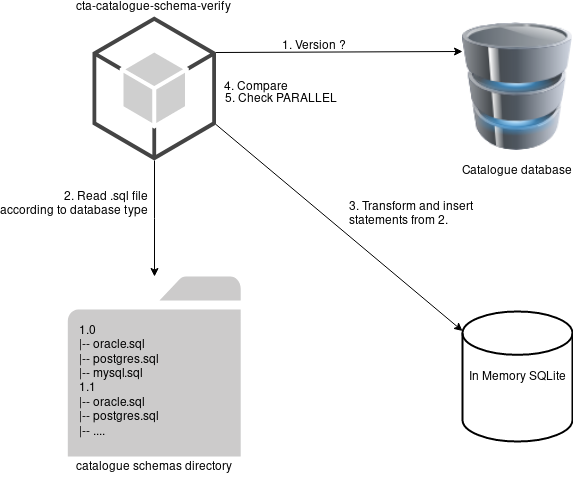
\includegraphics[keepaspectratio, height=0.7\textheight, width=0.7\textwidth]{schema-verify-operation.png}
    \end{figure}
  \end{center}
\end{frame}

\begin{frame}{The catalogue schema verification tool}
  \begin{itemize}
    \item The output
  \end{itemize}
  \begin{columns}
    \begin{column}{0.5\textwidth}
	  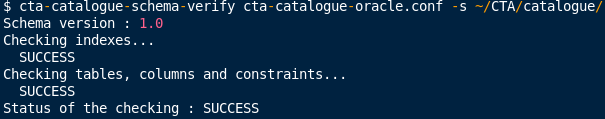
\includegraphics[keepaspectratio, height=1\textheight, width=1\textwidth]{SchemaVerifySuccess.png}
      \small{Schema verification SUCCESS}
    \end{column}
    \begin{column}{0.5\textwidth}
	  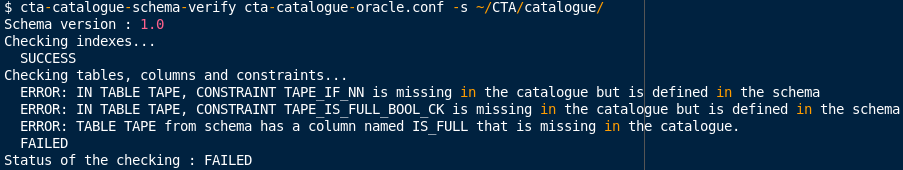
\includegraphics[keepaspectratio, height=1\textheight, width=1\textwidth]{SchemaVerifyRemovedColumn.png}
	  \small{Missing IS\_FULL column in table TAPE}
    \end{column}
  \end{columns}
  \begin{center}
	 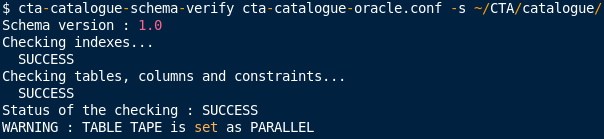
\includegraphics[keepaspectratio, height=0.7\textheight, width=0.7\textwidth]{ParallelTable.png}
	 \newline
	 \small{Table TAPE has been set as PARALLEL}
  \end{center}
\end{frame}

\begin{frame}{The catalogue schema verification tool}
	\begin{columns}
		\begin{column}{0.8\textwidth}
			\begin{itemize}
				\item What needs to be discussed
				\begin{itemize}
					\item Where do we put the folder containing all the versions of the schema ?
					\begin{itemize}
						\item Create a RPM of the cta-catalogue-schema-verify tool and stick the folder with it.
						
						$\Rightarrow$ This folder will be in the same place as the executable
						
						\item Other ideas ?
					\end{itemize}
				\end{itemize}
			\end{itemize}
		\end{column}
		\begin{column}{0.2\textwidth}
			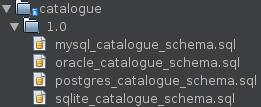
\includegraphics[keepaspectratio, height=1\textheight, width=1\textwidth]{SchemaFolder.png}
		\end{column}
	\end{columns}
\end{frame}

\section{The catalogue schema migration tool}
\begin{frame}{The database schema migration tool}
	\begin{itemize}
		\item Problem to solve
		\begin{itemize}
			\item Schema modifications $\Rightarrow$ new schema version !
			\begin{itemize}
				\item Schema version format : MAJOR.MINOR
				\item MAJOR changes ONLY if schema modifications are not backward compatible with previous schema version
			\end{itemize}
			\item How do we do catalogue schema migration from one version to the next one ?
		\end{itemize}
	\end{itemize}
\end{frame}

\begin{frame}{The catalogue schema migration tool}
	\begin{itemize}
		\item CASTOR's way of schema migration : PL/SQL file !
		\begin{itemize}
			\item 1. Check database schema version
			\item 2. Update tables, procedures, etc... (COMMIT after each update)
			\item 3. Recompile all procedures, triggers...
			\begin{itemize} 
				\item If all is successful, update a table UpgradeLog with status COMPLETE
				\item Else ROLLBACK current update and update UpgradeLog by increasing a failure counter, list the failed-to-compile objects
			\end{itemize}
		\end{itemize}
	\end{itemize}
\end{frame}

\begin{frame}{The catalogue schema migration tool}
	\begin{itemize}
		\item What would change between one schema version and the next one ?
		\begin{itemize}
			\item Creation/deletion/modification of tables, columns, constraints, sequences
			\item Data changes within tables
			\item Creation/deletion/modification of PL/SQL procedures
		\end{itemize}
	\end{itemize}
\end{frame}

\begin{frame}{The catalogue schema migration tool}
	\begin{itemize}
		\item The migration of the schema should
		% \adjustbox{minipage=1.11\textwidth, scale=0.9}{
		\begin{itemize}
			\item be idempotent
			\item do verification before each update (e.g: does a column exists before updating its type ?)
			\item be a step by step migration (one modification at a time)
			\item be rollbackable
			\item be traceable
			\item be easy to execute
		\end{itemize}
		\item The migration tool should be the same during the whole life of CTA
	\end{itemize}
\end{frame}

\begin{frame}{The catalogue schema migration tool}
	\begin{itemize}
		\item What kind of tool should we use to migrate the catalogue schema from one version to the next one ?
		\begin{itemize}
			\item Four ways
			\begin{itemize}
				\item Use a framework/language-dependant library
				\item Use an independent Database-Migration-Focused software
				\item Develop a tool ourselves
				\item Use simple PL/SQL scripts because after all, modifications will be little ones 
			\end{itemize}
		\end{itemize}
	\end{itemize}
\end{frame}

\begin{frame}{The catalogue schema migration tool}
	\begin{itemize}
		\item Use a framework/language-dependent library
		\begin{itemize}
			\item Python (alembic), Ruby (Active Record)
			\item No built-in support for Oracle databases
			$\Rightarrow$ We would need to use an ORM (Object-relational mapping) tool and plug a migration framework to it.
		\end{itemize}
	\end{itemize}
\end{frame}

\begin{frame}{The catalogue schema migration tool}
	\begin{itemize}
		\item Use an independent Database-Migration-Focused software
		\begin{itemize}
			\item Liquibase \href{https://www.liquibase.org/}{\beamergotobutton{Link}}
			\item Flyway \href{https://flywaydb.org/}{\beamergotobutton{Link}}
		\end{itemize}
	\end{itemize}
\end{frame}

\begin{frame}{The catalogue schema migration tool}
	\begin{itemize}
		\item Liquibase
		\begin{itemize}
			\item Open-source command-line tool based on Java. Apache v2 License
			\item Compatible with our 4 database types
			\item Easy-to-use : {\small \textit{liquibase --changeLogFile=migration1.0To1.1.sql update}}
			\item changeLogFile = sql file for doing the migration + Liquibase-related metadata
			\item Rollback changes
			\item Adds two Liquibase-related tables to the database
		\end{itemize}
	\end{itemize}
\end{frame}

\begin{frame}{The catalogue schema migration tool}
	\begin{itemize}
		\item Flyway
		\begin{itemize}
			\item Command-line tool based on Java. Apache v2 License
			\item Compatible with our 4 database types
			\item Easy-to-use : {\small \textit{flyway migrate}}
			\item Migration scripts have to be put in a specific folder. (Naming convention).
			\item Adds one history table to the database : flyway\_schema\_history
			\item A lot of functionalities only in PRO versions :-(
		\end{itemize}
	\end{itemize}
\end{frame}

\begin{frame}{The catalogue schema migration tool}
	\begin{itemize}
		\item Use simple PL/SQL scripts because after all, modifications will be little ones
		\begin{itemize}
			\item What do you think ?
		\end{itemize}
	\end{itemize}
\end{frame}

\begin{frame}{The catalogue schema migration tool}
	\begin{itemize}
		\item Conclusion
	\end{itemize}

	\begin{tabularx}{1\textwidth} { 
	  | >{\raggedright\arraybackslash}X 
	  | >{\raggedright\arraybackslash}X 
	  | >{\raggedright\arraybackslash}X | }
		\hline
		{\small Migration strategy} & {\small Pros} & {\small Cons} \\
		\hline
		{\tiny Framework/language-dependent lib} & {\tiny Use of exisiting lib to do migrations} & {\tiny No built-in support for Oracle} \\ 
		\hline
		{\tiny Database-Migration software} & {\tiny Easy migrations, well defined migration organization, Rollback} & {\tiny Timeline for our 4 databases support ? Changing technology might be difficult} \\ 
		\hline
		{\tiny Develop a tool ourselves} & {\tiny We depend on nobody except us} & {\tiny Time consuming. Safe ?} \\
		\hline
		{\tiny PL/SQL Scripts} & {\tiny Very easy to execute} & {\tiny Migration failure management} \\
	\end{tabularx}


	%\begin{center}
	%	\begin{tabular}{ | m{4cm} | m{5cm} | m{5cm} | } 
	%	 \hline
	%	 Migration strategy & Pros & Cons \\ 
	%	 \hline
	%	 Framework/language-dependent lib & Use of exisiting lib to do migrations & No built-in support for Oracle \\ 
	%	 cell7 & cell8 & cell9 \\ 
	%	 \hline
	%	\end{tabular}
	%\end{center}

\end{frame}

\backcover

\end{document}
